\input ../SlidePreamble
\input ../preamble


\begin{document}

{\Huge
  \centerline{\bf TTIC 31230,  Fundamentals of Deep Learning}
  \vfill
  \centerline{David McAllester, Autumn   2022}
  \vfill
  \centerline{\bf Contrastive Coding}
  \vfill
  \vfill


\slide{CLIP, January 2021, OpenAI}

CLIP: Contrastive Language-Image Pre-training.

\vfill
Trained on images and associated text (such as image captions or hypertext links to images) CLIP computes embeddings of text and embeddings of images
(``co-embeddings'') trained to capture the mutual information between the two.

\vfill
This is done with contrastive coding.

\slide{Contrastive Coding}


Consider a population distribution on pairs $\tuple{x,y}$ (such as images and associated text).

\vfill
We are interested in finding embedding functions $\enc_x$ and $\enc_y$ such that $\enc_x(x)$ and $\enc_y(y)$ are in the same embedding space
and capture the mutual information between $x$ and $y$.

\slide{CLIP Constrastive Coding}

\centerline{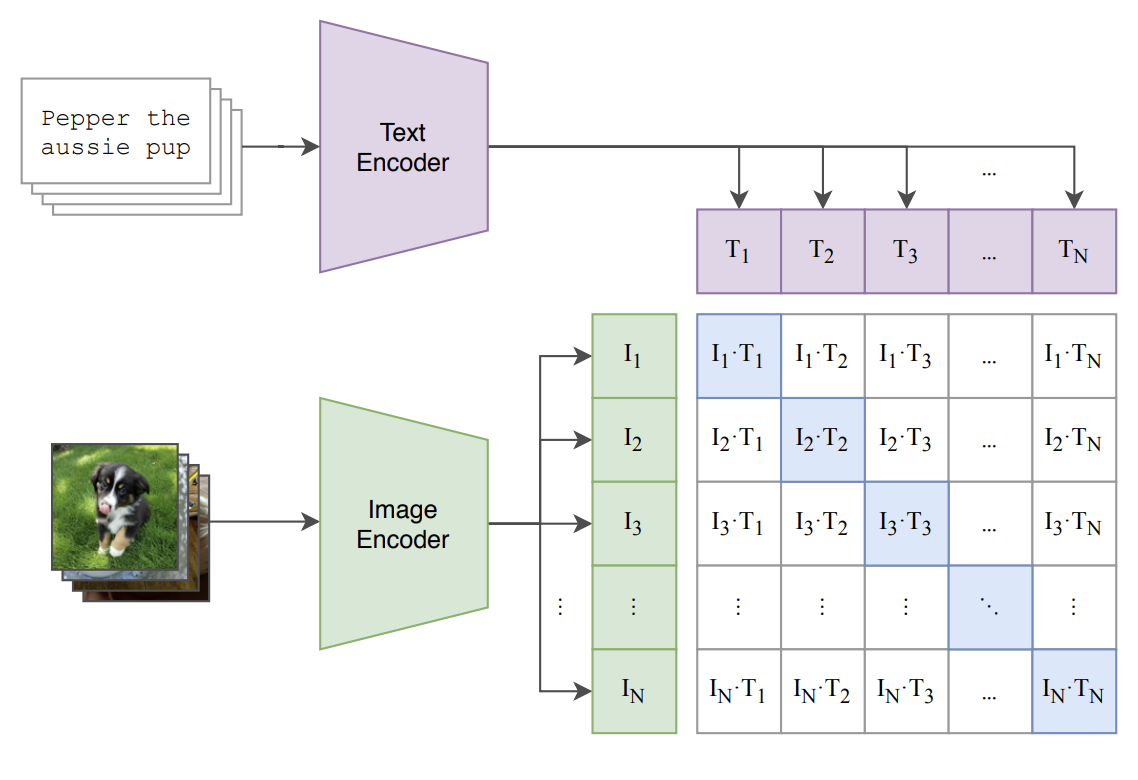
\includegraphics[height= 5in]{\images/CLIPTraining}}


\slide{Contrastive Coding}

\vfill
We draw pairs $(x_1,y_1), \ldots (x_n,y_n)$ from the population, and $i$ uniformly from $1$ to $N$.

\vfill
We then construct $(z_x,z_{y}^1,\ldots,z_y^N,i)$
by and setting $z_x = \enc_x(x_i)$ and $z_y^i = \enc_y(y_i)$.

\vfill
We then train a model to predict $i$.
\vfill
{\huge
\begin{eqnarray*}
\enc_x^*,\enc_y^* & = & \argmin_{\enc_x,\enc_y} \;E_{(z_x,z_y^1,\ldots,z_y^N,i)}\left[-\ln P(i|(z_x,z_y^1,\ldots,z_y^N)\right]
\end{eqnarray*}

\begin{eqnarray*}
P(i|z_x,z_y^1,\ldots z_y^N) & = & \softmax_i\; z_x^\top z_y^i
\end{eqnarray*}
}

\slide{The Contrastive Coding Theorem}

For any distribution on pairs $(z_x,z_y)$, if contrastive probabilities are computed by

{\huge
\begin{eqnarray*}
P(i|z_x,z_y^1,\ldots z_y^N) & = & \softmax_i\;s(z_x,z_y^i)
\end{eqnarray*}
}

then

{\huge
\begin{eqnarray*}
I(z_x,z_y) & \geq & \ln N - \;\;E_{(z_x,z_y^1,\ldots,z_y^N,i)}\left[-\ln P(i|(z_x,z_y^1,\ldots,z_y^N)\right]
\end{eqnarray*}
}

Chen et al., On Variational Bounds of Mutual Information, May 2019.

\slide{CLIP Image Classification}

\centerline{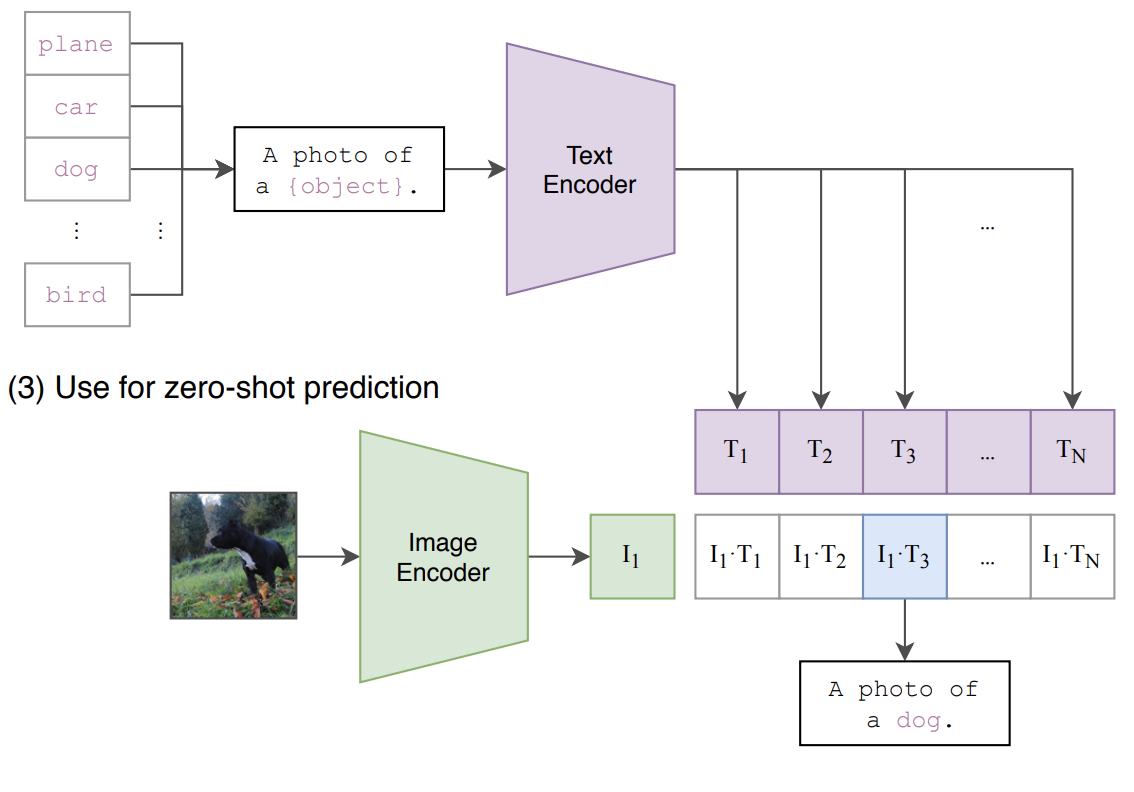
\includegraphics[height= 5in]{\images/CLIPClassifier}}

\slide{Zero-Shot Image Classification}

\centerline{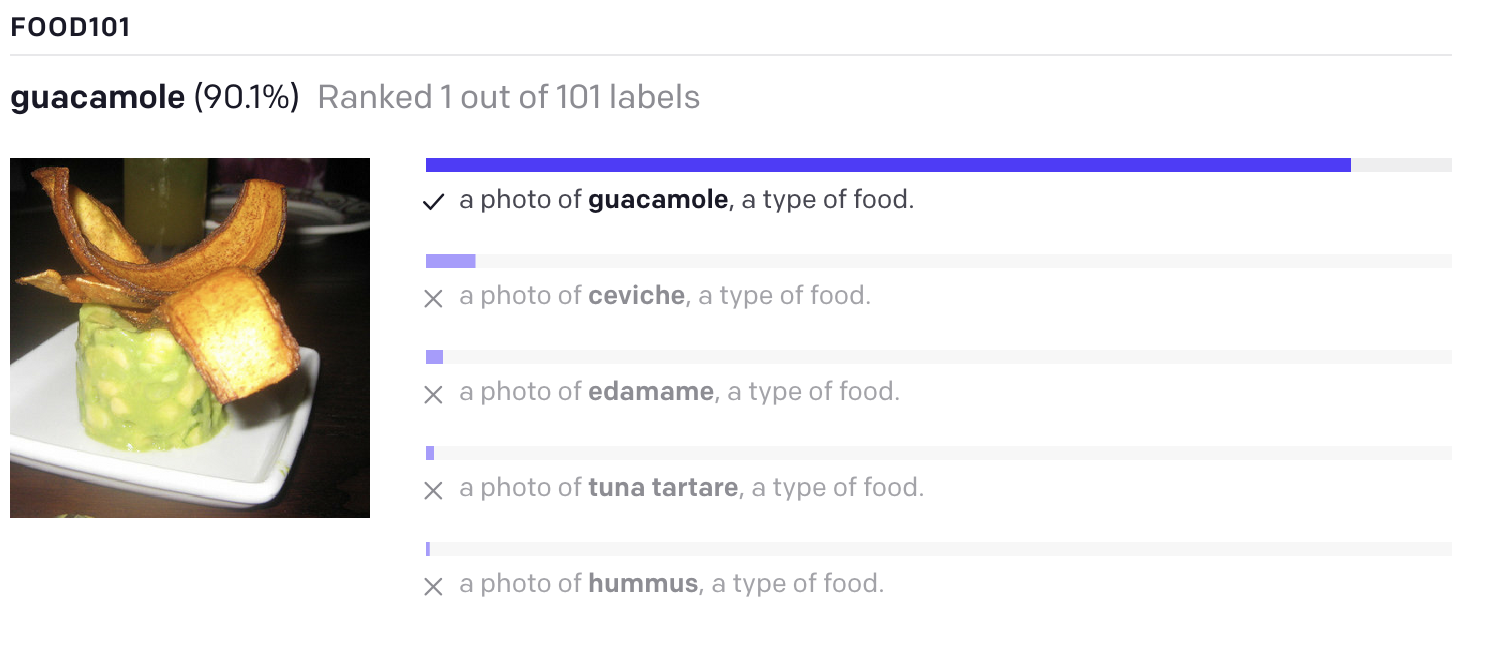
\includegraphics[width = 7in]{\images/CLIP0}}

\slide{Zero-Shot Image Classification}

\centerline{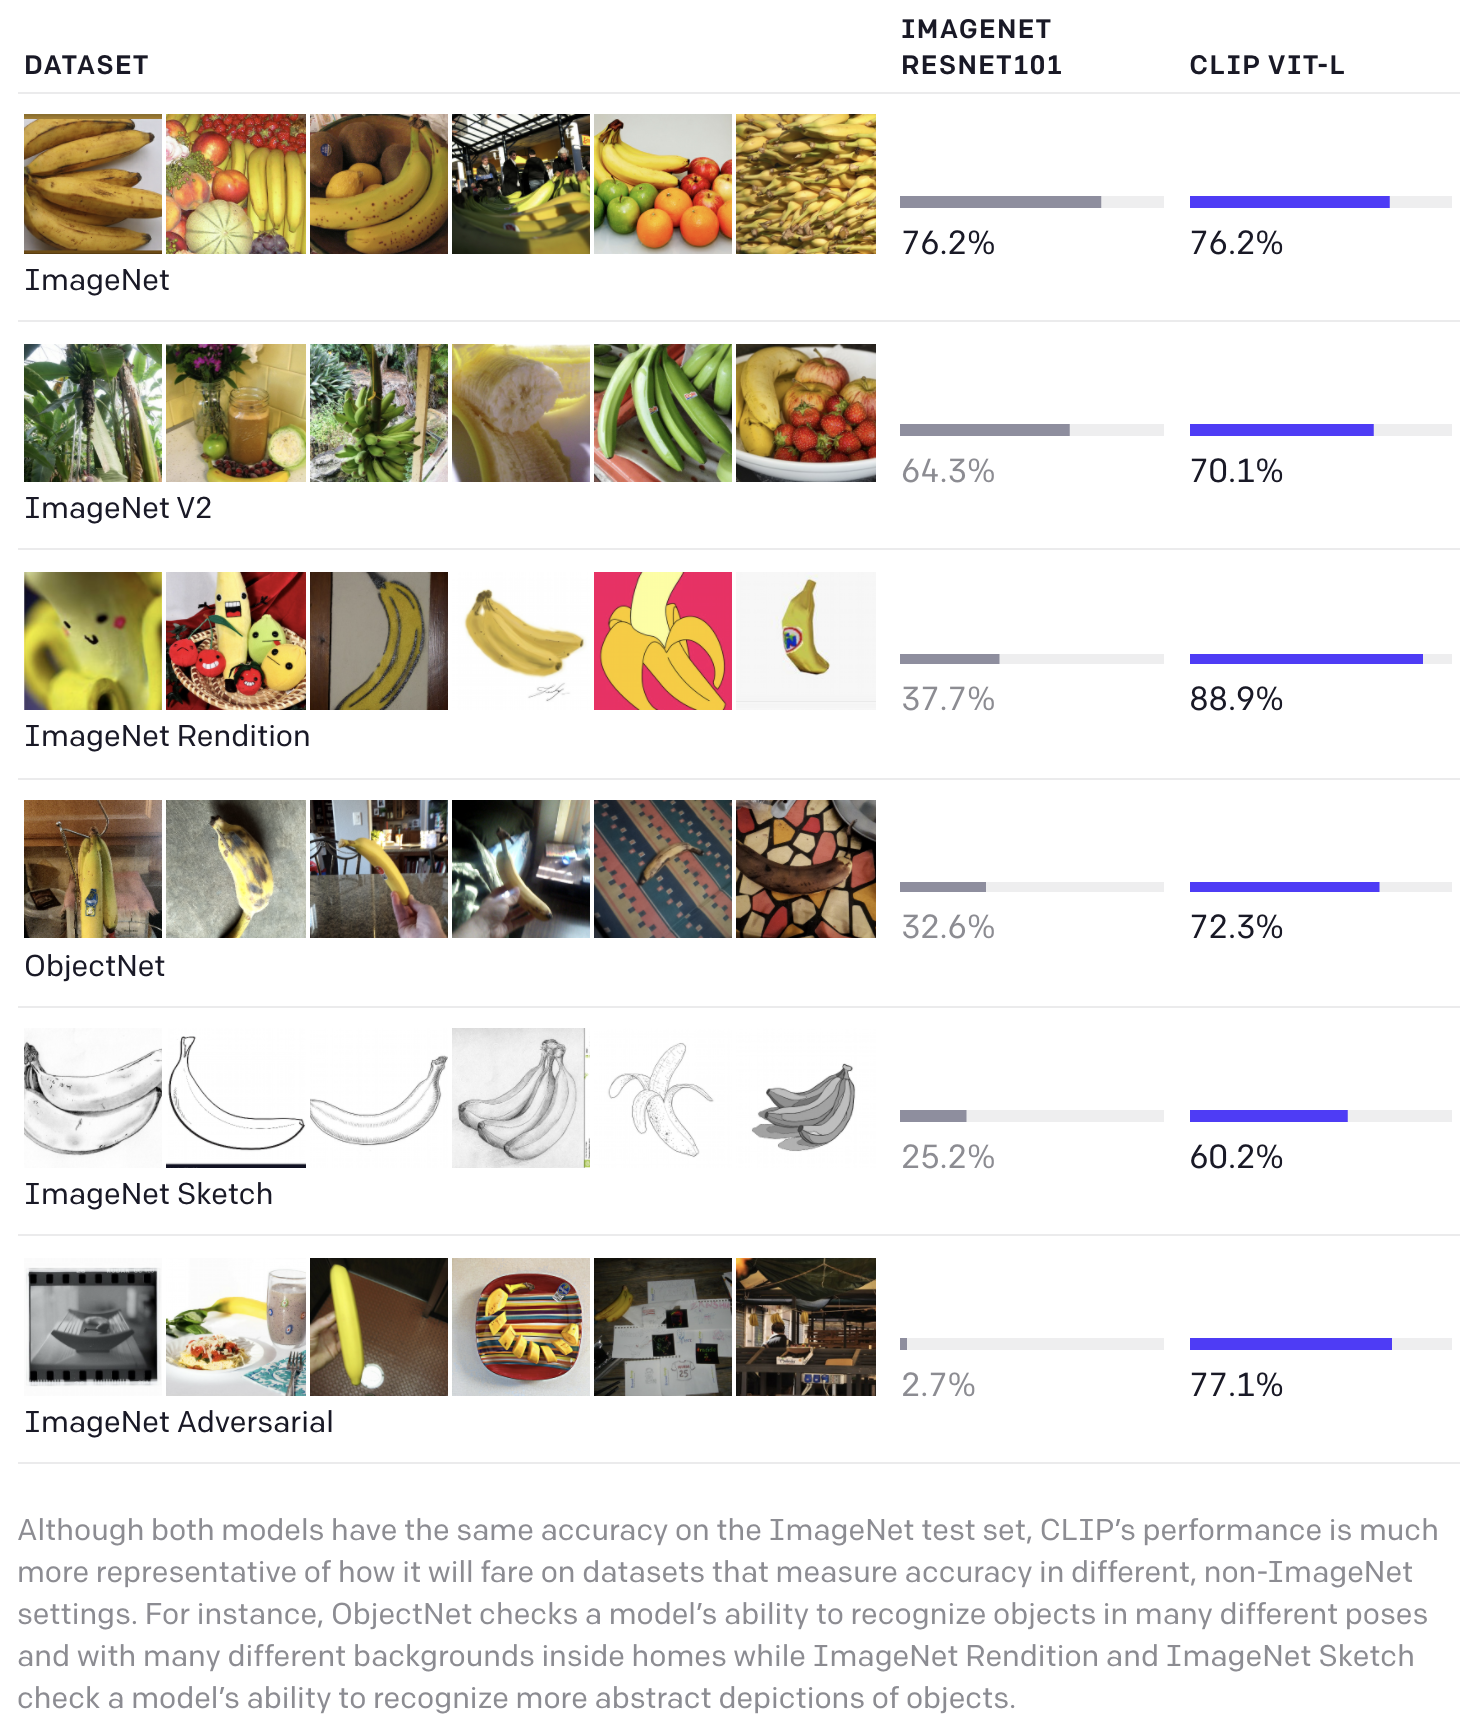
\includegraphics[height= 5in]{\images/CLIP1}}


\slide{Contrastive Coding for Speech}
\centerline{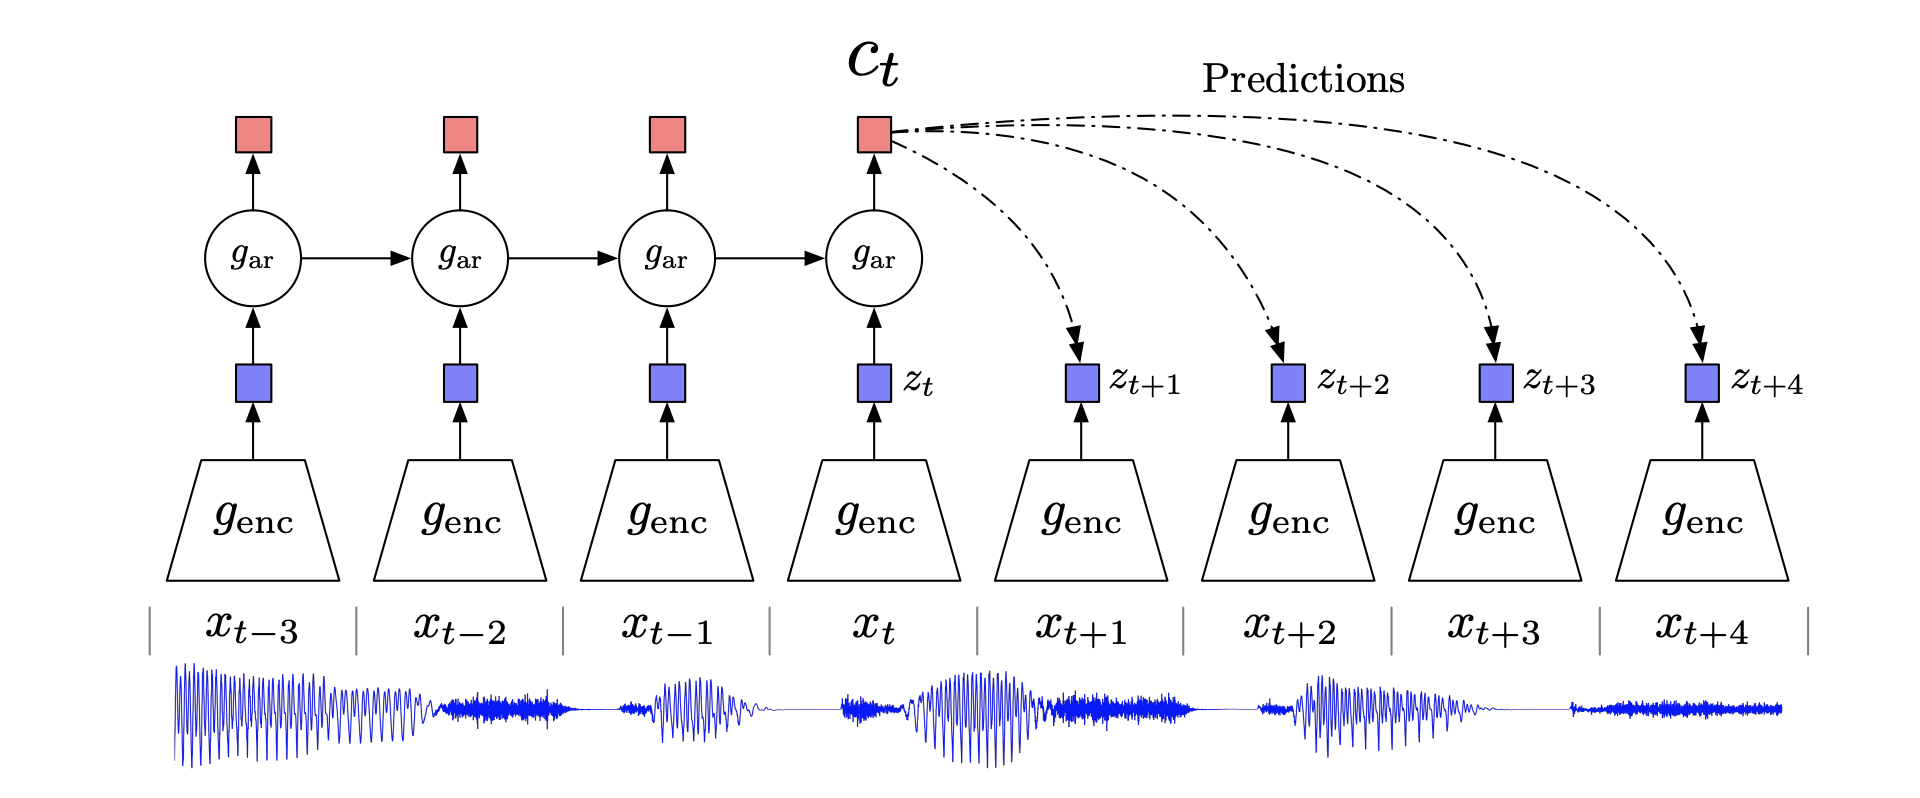
\includegraphics[width = 6 in]{\images/CPC}}
\centerline{\huge van den ORD et al. 2018}

\vfill
Consider the problem of learning phonetic representations of speech sounds.  In the figure each $z_t$ is a symbol representing the sound at time $t$.


\slide{Contrastive Coding for Speech}
\centerline{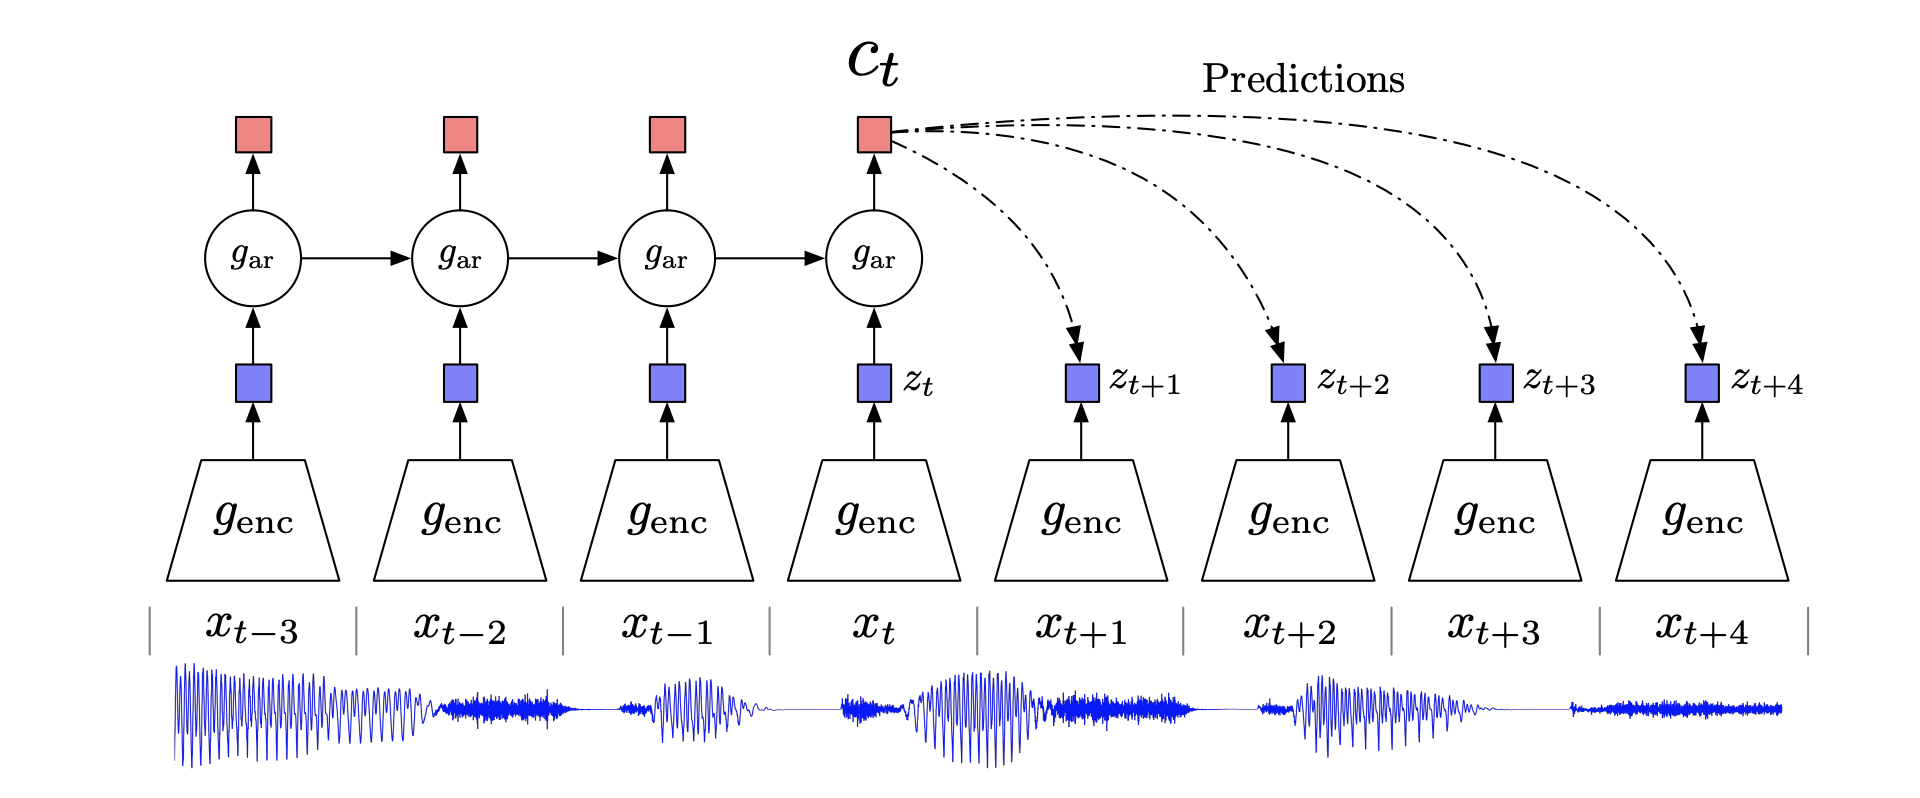
\includegraphics[width = 6 in]{\images/CPC}}
\centerline{\huge van den ORD et al. 2018}

\vfill
Here we want to train the networks so as to capture the mutual information between $c_t$ and $z_{t+i}$.

\vfill
This is done with the same contrastive loss function as in CLIP (and predates CLIP).

\slide{Contrastive Coding for Speech}
\centerline{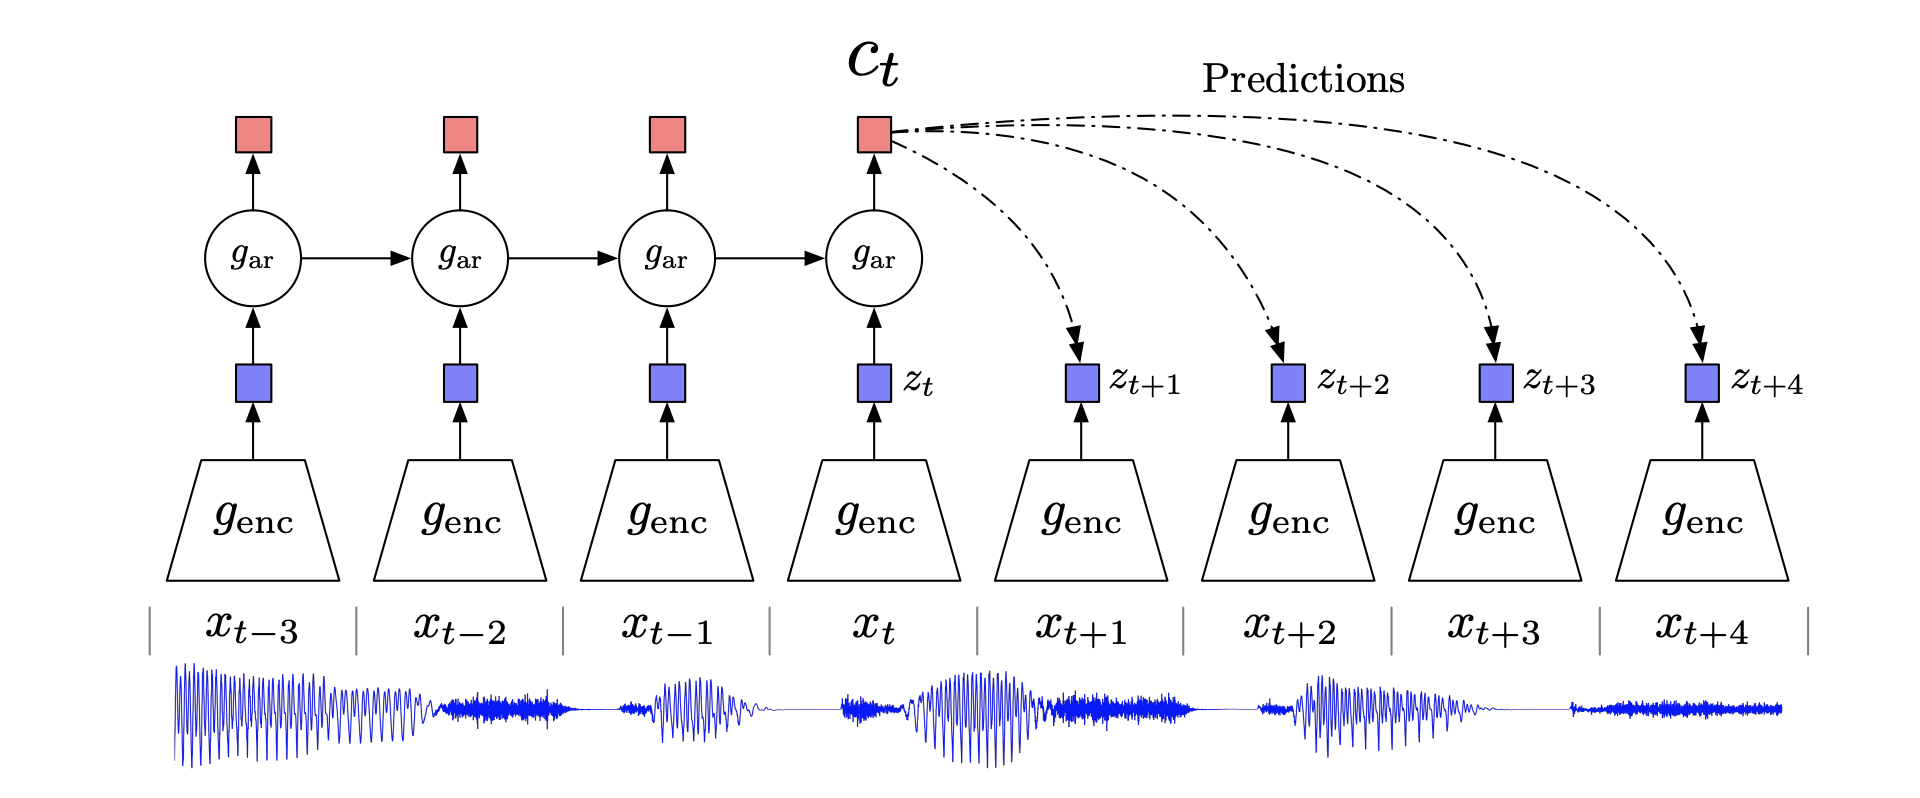
\includegraphics[width = 6 in]{\images/CPC}}
\centerline{\huge van den ORD et al. 2018}

\vfill
{\bf Unlike VAEs}, contrastive coding is about {\bf capturing mutual information}. There is no attempt to model the input speech sound.
Intuitively we want to separate signal from noise and avoid modeling noise.

\slide{wav2vec 2.0}

\vfill
Trained on 53k hours of {\bf unlabeled} audio they convert speech to a sequence of symbols they call ``pseudo-text units''.

\vfill
Using this pre-trained transcription of speech into pseudo-text they reduce the amount of labeled data needed for a given accuracy in speech recognition by a factor of 100.

\vfill
\centerline{\huge Baevski et al., 2020}

\slide{Augmentation Contrastive Coding for Images (SimCLR)}

(SimCLR:) A Simple Framework for Contrastive Learning of Visual Representations, Chen et al., Feb. 2020 (self-supervised leader as of February, 2020).

\vfill
They construct a distribution on pairs $\tuple{x,y}$ defined by drawing an image from ImageNet and then drawing $x$ and $y$ as random ``augmentations'' of the image.

\vfill
Augmentations include (among others) reflections, croppings, and changes in the color map.

\slide{Augmentation Contrastive Coding for Images (SimCLR)}

\vfill
They drawing an image from ImageNet and then draw $x$ and $y$ as random augmentations
of the same image.

\vfill
They then train a single coding function $\enc$ that applies to any augmentation and train the ecoding function by the
the contrastive coding objective objective.

\begin{eqnarray*}
\enc^* & = & \argmin_\enc \;E_{(z_x,z_y^1,\ldots,z_y^N,i)}\left[-\ln P(i|(z_x,z_y^1,\ldots,z_y^N)\right]
\end{eqnarray*}

\begin{eqnarray*}
P(i|z_x,z_y^1,\ldots z_y^N) & = & \softmax_i\; z_x^\top z_y^i
\end{eqnarray*}


\slide{Augmentation Contrastive Coding for Images (SimCLR}

The encoder is then used on images to define a feature vector for images.

\vfill
They then train a {\bf linear} imagenet classifier on the feature map defined by the encoder.

\vfill
This is called linear probing.

\slide{Augmentation Contrastive Coding for Images (SimCLR)}

\centerline{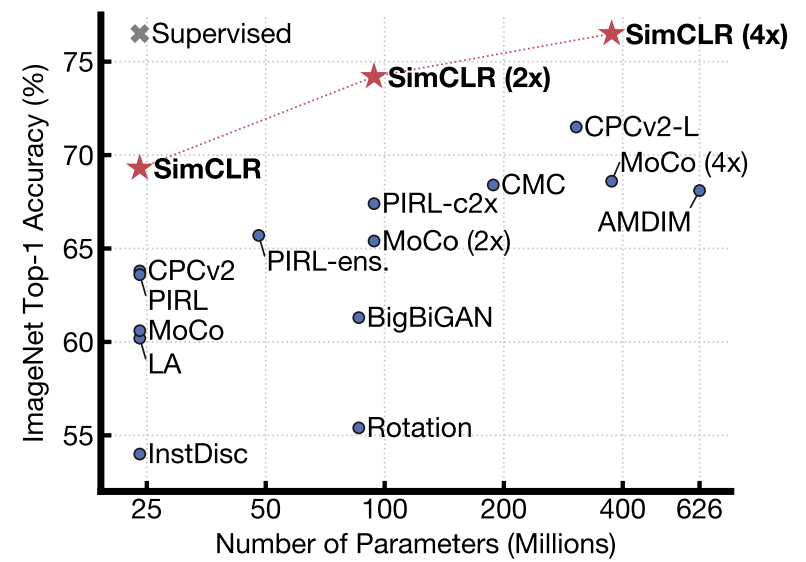
\includegraphics[height=3.5 in]{\images/SimCLR}}

\vfill
\centerline{\huge Chen et al. 2020}

\slide{A Weakness of Contrastive Coding}

{\huge
\begin{eqnarray*}
I(z_x,z_y) & \geq & \ln N - \;\;E_{(z_x,z_y^1,\ldots,z_y^N,i)}\left[-\ln P(i|(z_x,z_y^1,\ldots,z_y^N)\right]
\end{eqnarray*}
}

The discrimination problem is too easy.

\vfill
The guarantee can never be stronger than $\ln N$ where $N$ is the number of choices in the discrimination task.

\slide{Contrastive Cluster Assignments}

For a population on pairs $\tuple{x,y}$ we might consider the following training objective.

\vfill
\begin{eqnarray*}
\enc_x^*,\enc_y^* & = & \argmax_{\enc_x,\enc_y} \; I(z_x,z_y) \;\;\;z_x = \enc_x(x),\;z_y = \enc_y(y)
\end{eqnarray*}

\vfill
Unfortunately this has a degenerate solution of $\enc_x(x) = x$ and $\enc_y(y) = y$.

\slide{Contrastive Cluster Assignments}

To block the degenerate solution we first rewrite the mutual information objective function.

\vfill
\begin{eqnarray*}
\enc_x^*,\enc_y^* & = & \argmax_{\enc_x,\enc_y} \; I(z_x,z_y) \\
\\
&= & \argmax_{\enc_x,\enc_y}\; H(z_y) - H(z_y|z_x) \\
\\
&= & \argmin_{\enc_x,\enc_y}\; H(z_y|z_x) - H(z_y)
\end{eqnarray*}

\slide{Contrastive Cluster Assignments}

\begin{eqnarray*}
\enc_x^*,\enc_y^* & = &  \argmin_{\enc_x,\enc_y}\; H(z_y|z_x) - H(z_y)
\end{eqnarray*}

\vfill
We can block the solution of $\enc_y(y) = y$ by requiring that $\enc_y(y)$ is a symbol from a finite vocabulary of size $K$.

$$H(z_y) \leq \ln K$$

\vfill
We can then allow $\enc_x(x) = x$.

\slide{Direct MI Coding}

\begin{eqnarray*}
\enc_x^*,\enc_y^* & = &  \argmin_{\enc_x,\enc_y}\; H(z_y|z_x) - H(z_y)
\end{eqnarray*}

\vfill
We can train a model $\pred$ to predict $z_y$ from $z_x$ and train on cross-entropy loss.

\vfill
We can estimate $H(z_y)$ from an empirical histogram over the symbols and int


\slide{Direct MI Coding}

$$\enc_x^*,\enc_y^*,\Psi^* = \argmin_{\enc_x,\enc_y,\Psi} \; E_{(x,y)\sim \pop}\left[-\ln P_\Psi(z_y|z_x) + \ln \hat{P}(z_y)\right]$$

\vfill
where $\hat{P}(z_y)$ is an estimate (perhaps an exponential moving average) of the probability of $z_y$ over the draw of $(x,y) \sim \pop$.

\slide{Direct MI Coding Theorem}

$$\enc_x^*,\enc_y^*,\Psi^* = \argmin_{\enc_x,\enc_y,\Psi} \; E_{(x,y)\sim \pop}\left[-\ln P_\Psi(z_y|z_x) + \ln P(z_y)\right]$$

\vfill
\begin{eqnarray*}
I(z_x,z_y) & \geq & H(z_y) - \hat{H}(z_y|z_x) \\
\\
\hat{H}(z_y|z_x) & = & E_{(x,y)\sim \pop}\left[-\ln P_\Psi(z_y(y)|z_x(x)\right]
\end{eqnarray*}

\slide{Direct MI Coding Theorem}

For $H(z_y) = \ln K$ where $K$ is the number of symbols, and $\hat{H}(z_y|z_x) = 0$ we get

$$I(z_x,z_y) \geq \ln K$$

\vfill
Which typically improves significantly on the best possible bound $I(z_x,z_y) \geq \ln N$ from CPC.

\slide{ SwAV}

SwAV uses direct MI coding rather than SimCLR's CPC.


\centerline{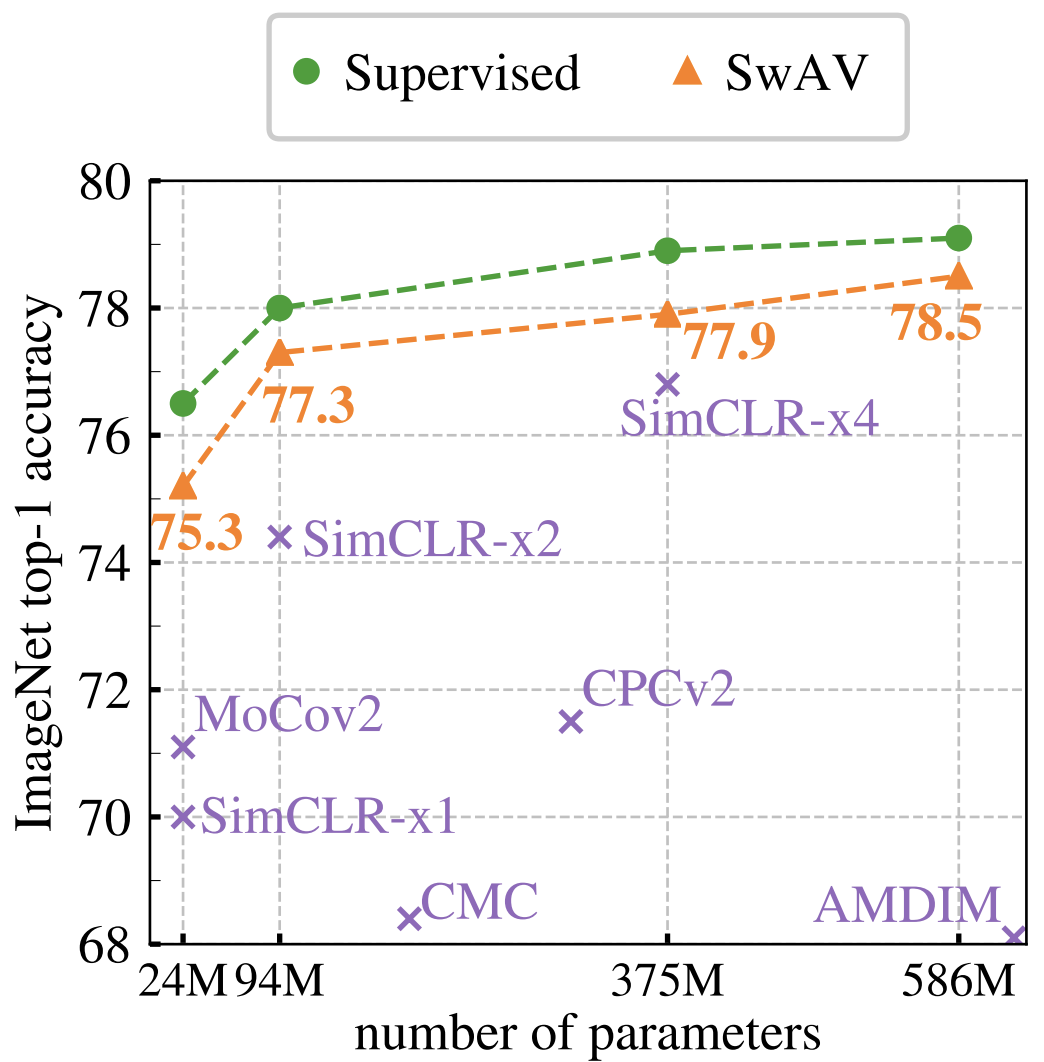
\includegraphics[width = 3.5in]{\images/SwAV}}

\centerline{\huge Caron et al. 2021}

\slide{END}

}
\end{document}


\slide{END}

}
\end{document}

